\documentclass[../main/main.tex]{subfiles}


\begin{document}

\section{March 3rd, 2021}
\subsection{Preoperational Stage}
\index{preoperation stage}
The preoperational stage occurs from ages 2-7 years old. During this stage,, the child learns to use and to represent objects by symbols. However, preoperational thought is still illogical, namely they demonstrate:
\begin{itemize}
\item Egocentricism
\item Centration
\item Irreversibility
\end{itemize}

\begin{description}
  \item[Egocentricism:] The belief that everyone sees and experiences the world the way he/she does. This indicates the inability to take the perspective of others. \index{egocentricism}
        \begin{remark}
This is different from being selfish, as they are simply unable to see from others perspectives.
        \end{remark}
        A typical task to test is called the three-mountains task. Where the child is asked to describe what they see. Then they switch places and the child is asked again what they see. Afterwards, the experimenter asks the child ``What do I see?'' Usually the child will say the same thing as before.

        \begin{figure}[htpb]
          \centering
          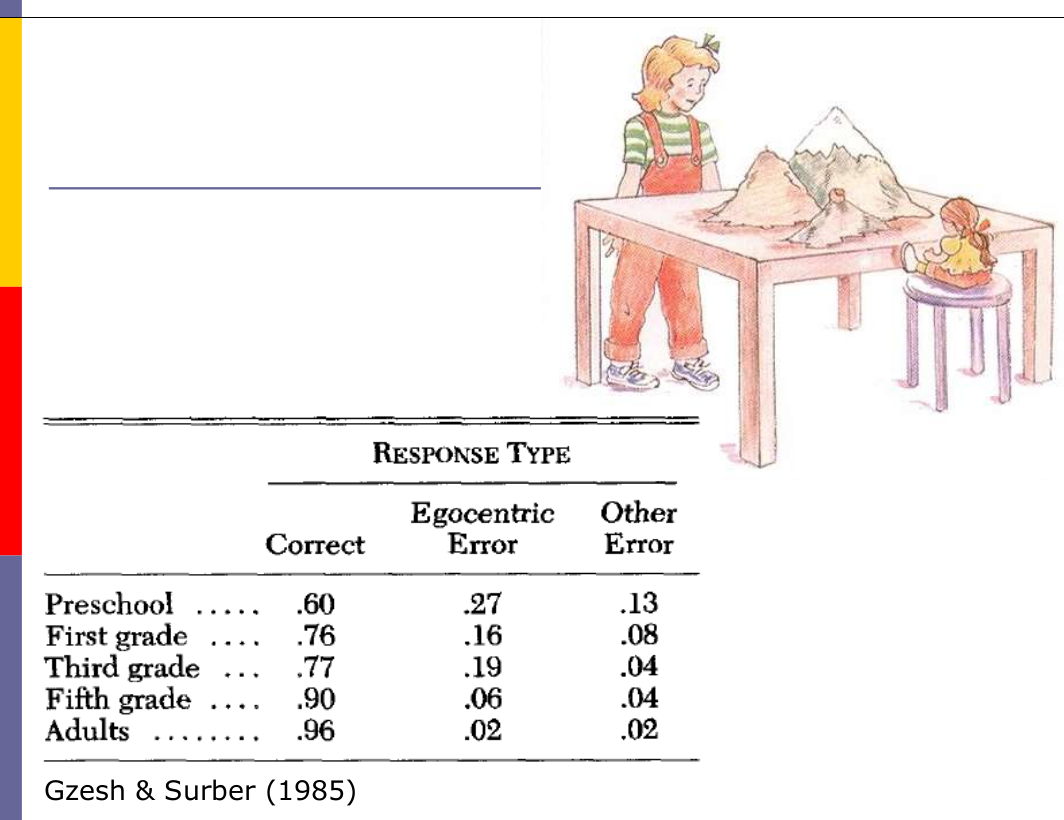
\includegraphics[width=0.8\textwidth]{../images/3-mount.png}
          \caption{Three Mountain Task}
          \label{fig:3mount}
        \end{figure}\index{three mountain task}

\item[Centration:] The tendency to think of the world in terms of one variable at a time. For example, animism, which is ascribing lifelike qualities to inanimate objects.\index{cnetration}
\item[Irreversibility:] The inability to mentally reverse actions or ideas. This can be demonstrated in conservation tasks, where the child thinks that the amount of something changes with the appearance. One example of a conservation task is that of the conservation of liquid in Figure \ref{fig:3-3-liq}. Children in the preoperational stage often thought that the taller glass have more water.\index{irreversibility}\\

\begin{figure}[h!]
  \centering
  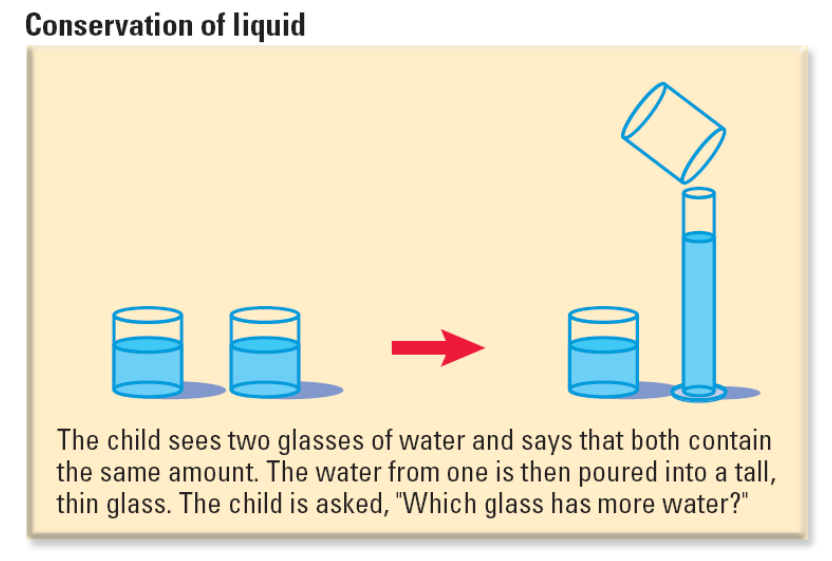
\includegraphics[width=0.8\textwidth]{../images/3-3-liq}
  \caption{Conservation of Liquid Task}
  \label{fig:3-3-liq}
\end{figure}

        Other conservation tasks

\end{description}
\subsubsection{Theories of Mind} \index{theories of mind}
Another developmental milestone that occurs in the preoperational stage is that of \vocab{Theories of Mind (TOM)}. This is the awareness and understanding of their own mental processes and those of other people. Piaget believes that children younger than 4 do not have theories of mind. Some indicators that the child has developed TOM include:
\begin{description}
  \item[False Beliefs:] The understanding that people can believe things that turn out to be false. One example is that of the Sally-Anne task, as shown in Figure \ref{fig:3-3-sally}.

    \begin{figure}[h!]
      \centering
      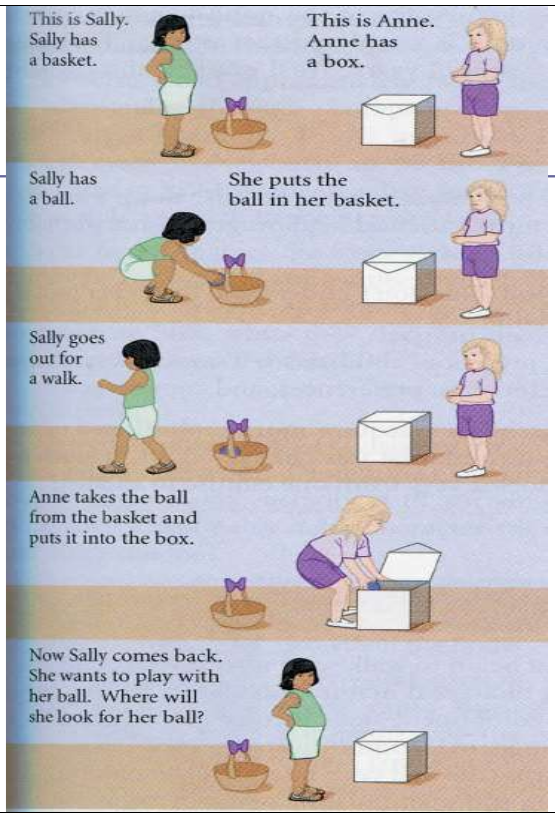
\includegraphics[width=0.6\textwidth]{../images/3-3-sally}
      \caption{Sally-Anne Task}
      \label{fig:3-3-sally}
    \end{figure}\index{Sally-Anne task}

        Children are told the situation and are asked where Sally would look for her ball. Children who have not developed TOM would say that it is in the box, as they do not understand that people can have false beliefs. In order to pass this task, they must understand that:
        \begin{itemize}
          \item People's beliefs are abased on their own knowledge
                \item People's behavior can be predicted by their beliefs
          \item Other people's mental representation of the situation can be different from his/her own
                \item Beliefs can differ from reality
        \end{itemize}
        \begin{remark}
          There are some influences on TOM development, including:
          \begin{itemize}
            \item Sibling advantage - Children with older siblings are likely to master false-belief understanding earlier than their peers
            \item Language skills - Children with knowledge of words for feelings, desires, and thoughts (e.g. want, think, remember, etc.) have TOM earlier than peers. This is why preschool-aged girls master TOM tasks before boys.
          \end{itemize}
        \end{remark}
  \item[Appearance vs. Reality:] The understanding of the distinction between what \textit{seems} to be and what \textit{is}. One example is the sponge-rock test, where a sponge is painted to look like a rock. They are then asked:
        \begin{itemize}
\item ``What does it look like?''
                \item ``what is it really?''
        \end{itemize}
        Children under 5 tend to respond with the same thing. Older children are able tell the distinction.
  \item[Fantasy vs Reality:] The understanding of the distinction between fantasy and reality.
        \begin{remark}
Children under 5 might think that mickey mouse is real. This is an example of the confusion between fantasy and reality.
        \end{remark}
        \begin{remark}
          However, the line between fantasy and reality may still be blur. Children are presented with two boxes, one with an imaginary bunny and the other with an imaginary lion. They were then asked which box they would like to touch. Even though neither are real, children prefer
        \end{remark}
\end{description}
To summarize, in the preoperational stage, children undergo the \textbf{increase in proficiency in the use of symbols.}\\

One challenge to Piaget's theory in the preoperational stage is related to the three-mountains task:
\begin{itemize}
  \item The three-mountains task may be limited by their language ability, as it is too difficult for the young child to properly express.
  \item To fix this, the child is asked to point to pictures instead of verbally expressing themselves.
        \item They found that children as young as 2-3 have some ability to view from another angle.
\end{itemize}

\subsection{Concrete Operations Stage}
\begin{itemize}
\item
The concrete operations stage happens from 7-12 years old.
  \item The child has eliminated egocentricism
\item The child is also able to master conservation, meaning that the understand that quantities is unrelated to arrangement or appearance of objects.
  \item The child is also able to perform classifications. For example:
       \begin{description}
         \item[Multiple Classification:] The ability to classify objects based on two or more dimensions.
         \item[Hierarchical Classification:]
               The understanding that subordinate classes of objects are included in super-ordinate classes
               \begin{example}
Are there more apples or more fruits.
               \end{example}
       \end{description}
  \item The child is also able to understand transitivity.
\begin{definition}[\vocab{Transitivity}]
        The understanding of the logical relationships among elements in a serial order\index{transitivity}
\end{definition}
        \begin{example}
If A is taller than B, and B is taller than C. Then A is taller than C.
        \end{example}
  \item The child is also able to understand seriation.
        \begin{definition}
[\vocab{Seriation}] The ability to use a rule to put an array of objects in order.\index{seriation}
        \end{definition}
        \begin{example}
Arrange sticks in arranging order. Children under the age of 7 found difficulty in this.
        \end{example}
  \item The most important developmental milestone in this stage is inductive logic.
        \begin{definition}[\vocab{Inductive Logic}] General principles are inferred from specific experiences.\index{inductive logic}
        \end{definition}
        \begin{example}
After touching ice and seeing it is cold, and that all ice they touch is cold, they can infer the general principle that ice is cold.
        \end{example}
\end{itemize}
\begin{figure}[h!]
  \centering
  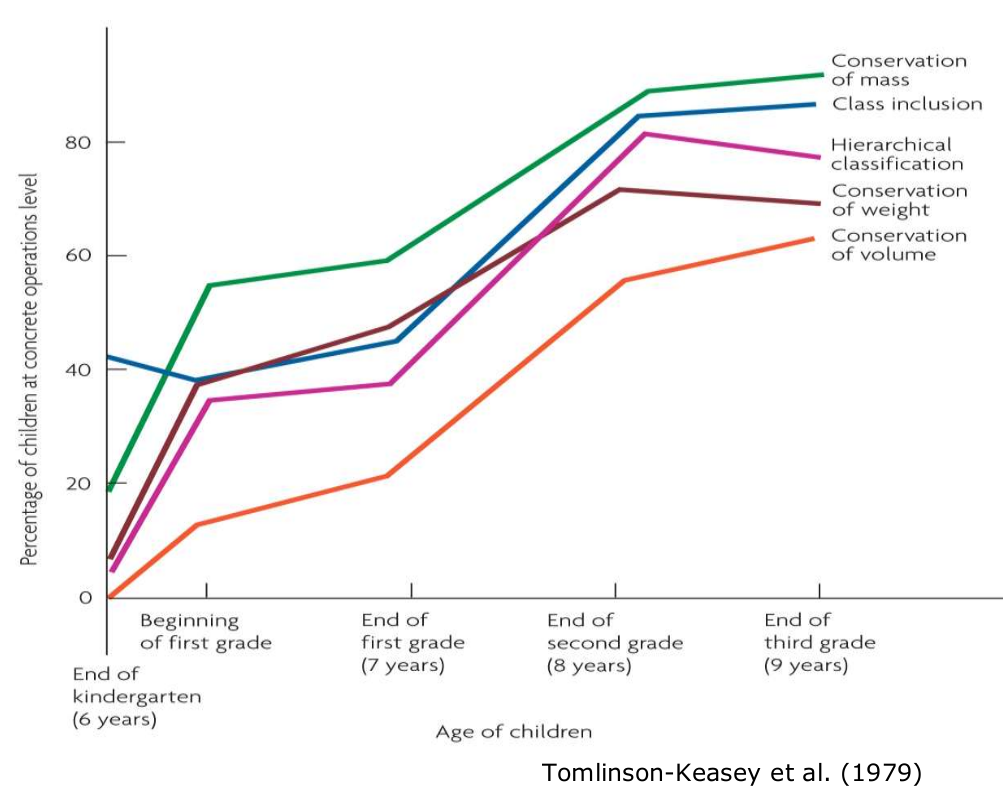
\includegraphics[width=0.8\textwidth]{../images/3-3-con}
  \caption{Research Done About the Mastery of Conservation}
\end{figure}

In summary, in the concrete operations stage, \textbf{children are better capable of thinking logically about objects and events in the real world.}

\subsection{Formal Operations Stage}
\index{formal operations stage}
\begin{itemize}
  \item Occurs from 12-15 years old
\item The individual moves beyond concrete experiences and begin to think abstractly.
  \item One milestone is hypothetical-deductive reasoning
        \begin{definition}
[\vocab{Hypothetical-Deductive Reasoning}] The ability to derive conclusions from hypothetical premises.\index{hypothetical-deductive reasoning}
        \end{definition}
        \begin{example}
If you hit a glass with a feather, it breaks. Children in the concrete operational stage would still operate on their experience, i.e. nothing will happen when it hits the glass.
        \end{example}
  \item Another development in this stage is problem solving.
        \begin{definition}[\vocab{Problem Solving}] THe ability to search methodically for the answer.
        \end{definition}
        \begin{example}
Which factors determine how fast a pendulum swing? How can we test this?
        \end{example}
\end{itemize}
One challenge to Piaget is that he overestimates the cognitive skills of many adults. He believes that all adults are able to master certain tasks when they reach formal operations stage.
\begin{example}
Some adults might still have egocentricism.
\end{example}

\end{document}
